% !TeX root=main.tex
\chapter{نتایج}
%\thispagestyle{empty} 
\label{chap:results}
% \subsection{تبعیت از روند آزمایش}
% از میان
% ارائهٔ داده‌ها، نتایج، تحلیل و تفسیر اولیهٔ آنها در این فصل ارائه می‌شود. در ارائهٔ نتایج با توجه به راهنمای كلی نگارش فصل‌ها، تا حد امکان، ترکیبی از نمودار و جدول استفاده شود. با توجه به حجم و ماهیت تحقیق و با صلاحدید استاد راهنما، اين فصل می‌تواند تحت عنوانی دیگر بیاید. در صورتی که حجم داده‌ها زیاد باشد، بهتر است به صورت نمودار یا در قالب ضمیمه ارائه نشده و فقط نمونه‌ها در متن آورده شود. در این فصل باید به سوالات تحقیق، عطف به یافته‌های محقق، پاسخ داده شود. اگر تحقیق دارای آزمون فرض باشد، پذیرش یا عدم پذیرش فرضیه‌ها در این فصل گزارش می‌شود. این فصل حدود ۴۰ صفحه است.

% در این بخش به سوالات تحقیق، بر اساس داده‌ها و یافته‌های محقق، پاسخ داده می‌شود. داده‌ها با فرمت مناسبی ارائه می‌شوند؛ مدل (ها) اجرا شده و نتیجه آن مشخص می‌شود.
% \subsection{سیاهه ارزش‌گذاری مجموعه‌داده}
\section{پیش پردازش داده و نتایج اولیه}
داده‌های جمع‌آوری شده که به صورت یک فایل با فرمت 
\lr{json}
بر روی سرور ذخیره شده بودند، توسط کتابخانه‌های پردازش داده زبان برنامه نویسی پایتون 
\lr{numpy}
\!،
\lr{pandas}
 و
\lr{scipy}
پردازش شدند. از تعداد $\InitialSampleSizeTotal$
نفری که وارد اولین صفحه شده بودند،
$\LandingPageDrops$
نفر بلافاصله و بدون زدن دکمه 
\textit{شروع آزمایش}
\!، 
آزمایش را ترک کردند.
$\GlobalConsentDrops$
نفر پس از مشاهده صفحه دوم
\!(
    اعلام رضایت
    ) 
    بدون زدن دکمه
    \textit{تایید}
    خارج شدند.
    
$\CleandDataDFForPlotsSizeFemalePlusMale$
چهار بخش ابتدایی آزمایش شامل
\textit{معرفی اولیه}،
\textit{پرسشنامه اول}،
\textit{پرسشنامه دوم} و
\textit{معرفی ثانویه}
را کامل کرده بودند.
از این میان، داده‌هایی که فاقد اطلاعات بودند و یا اطلاعات وارد شده توسط آزمودنی
مانند نام و نام‌خانوادگی و شماره تلفن‌ها مخدوش و غیر قابل تشخیص بودند، پاکسازی شدند. 

از این میان داده های افرادی که مشخصات وارد شده توسط آنها مخدوش و غیر صحیح 
بودند، جذف شدند. همچنین
$\ValidParticipantsWithBogusPhoneSize$
 نفر  از شرکت کنندگان با وجود اینکه 
بخش های مختلف آزمایش را به درستی انجام داده بودند، به این دلیل که شماره تلفن نامعتر
برای فرد معرفی شده در بخش‌های 
\textit{معرفی اولیه}
و
\textit{معرفی ثانویه}
وارد کرده بودند. همچنین
$1$
نفر دیگر نیز به جای شماره تلفن، ایمیل خود را وارد کرده بود. داده‌های این افراد نیز از نتایج جذف شدند
و در نهایت 
$\CleandDataDFForPlotsMinusBogusSize$
باقی ماندند که از این مجموعه داده برای انجام سنجش‌های آماری استفاده شد.

\section{سیاهه ارزش‌گذاری مجموعه‌داده}
در این پژوهش از
% سیاهه ارزش‌گذاری مجموعه‌داده
{\textit{\gls{Dataset valuation invetory}}}
که یک
{\textit{\gls{The researcher made a questionnaire}}}
است برای اندازه‌گیری
\gls{Attitude}
نسبت به ارزش دسته‌های مختلف اطلاعات شخصی، استفاده شده است.
\textit{\gls{Trial}}
هر یک از آزمودنی‌ها در هر
\textit{\gls{Trial}}
به
\textit{\gls{Dataset}}
ارائه شده عددی از بازه صفر تا ۱۰۰ نسبت داده است. این عدد به عنوان مقیاسی از ارزش ذهنی
\textit{\gls{Subjective value}}
دسته‌ای از اطلاعات که
\textit{\gls{Trial}}
به آن تعلق دارد، تلقی می‌شود
زمان شروع
\textit{\gls{Online survey}}
\textit{\gls{Consent}}
آزمودنی‌ها به طور تصادفی و از طریق کد
\textit{\gls{JavaScript}}
اجرا شده در
\textit{\gls{Browser}}
به دو دسته تقسیم شدند.
\section{ویژگی‌های نمونه}
تعداد کل آزمودنی ها
$\InitialSampleSize$
نفر،
با بازه سنی
\ageMin
تا
\ageMax
و
میانگین
\sampleAgeMean
و انحراف استاندارد
\sampleAgeSD
بود
\!.
از این میان
\SampleSizeMale
نفر مذکر و
\SampleSizeFemale
مونث بودند.
تعداد
\SampleSizeSexualityNoAnswer
نیز از بین گزینه‌های مربوط به جنسیت گزینه عدم تمایل به پاسخگویی را انتخاب کردند
(
تصویر \label{fig:sexualityAgainstPopulation}
)
\!.

% \begin{figure}[ht]
%     \centerline{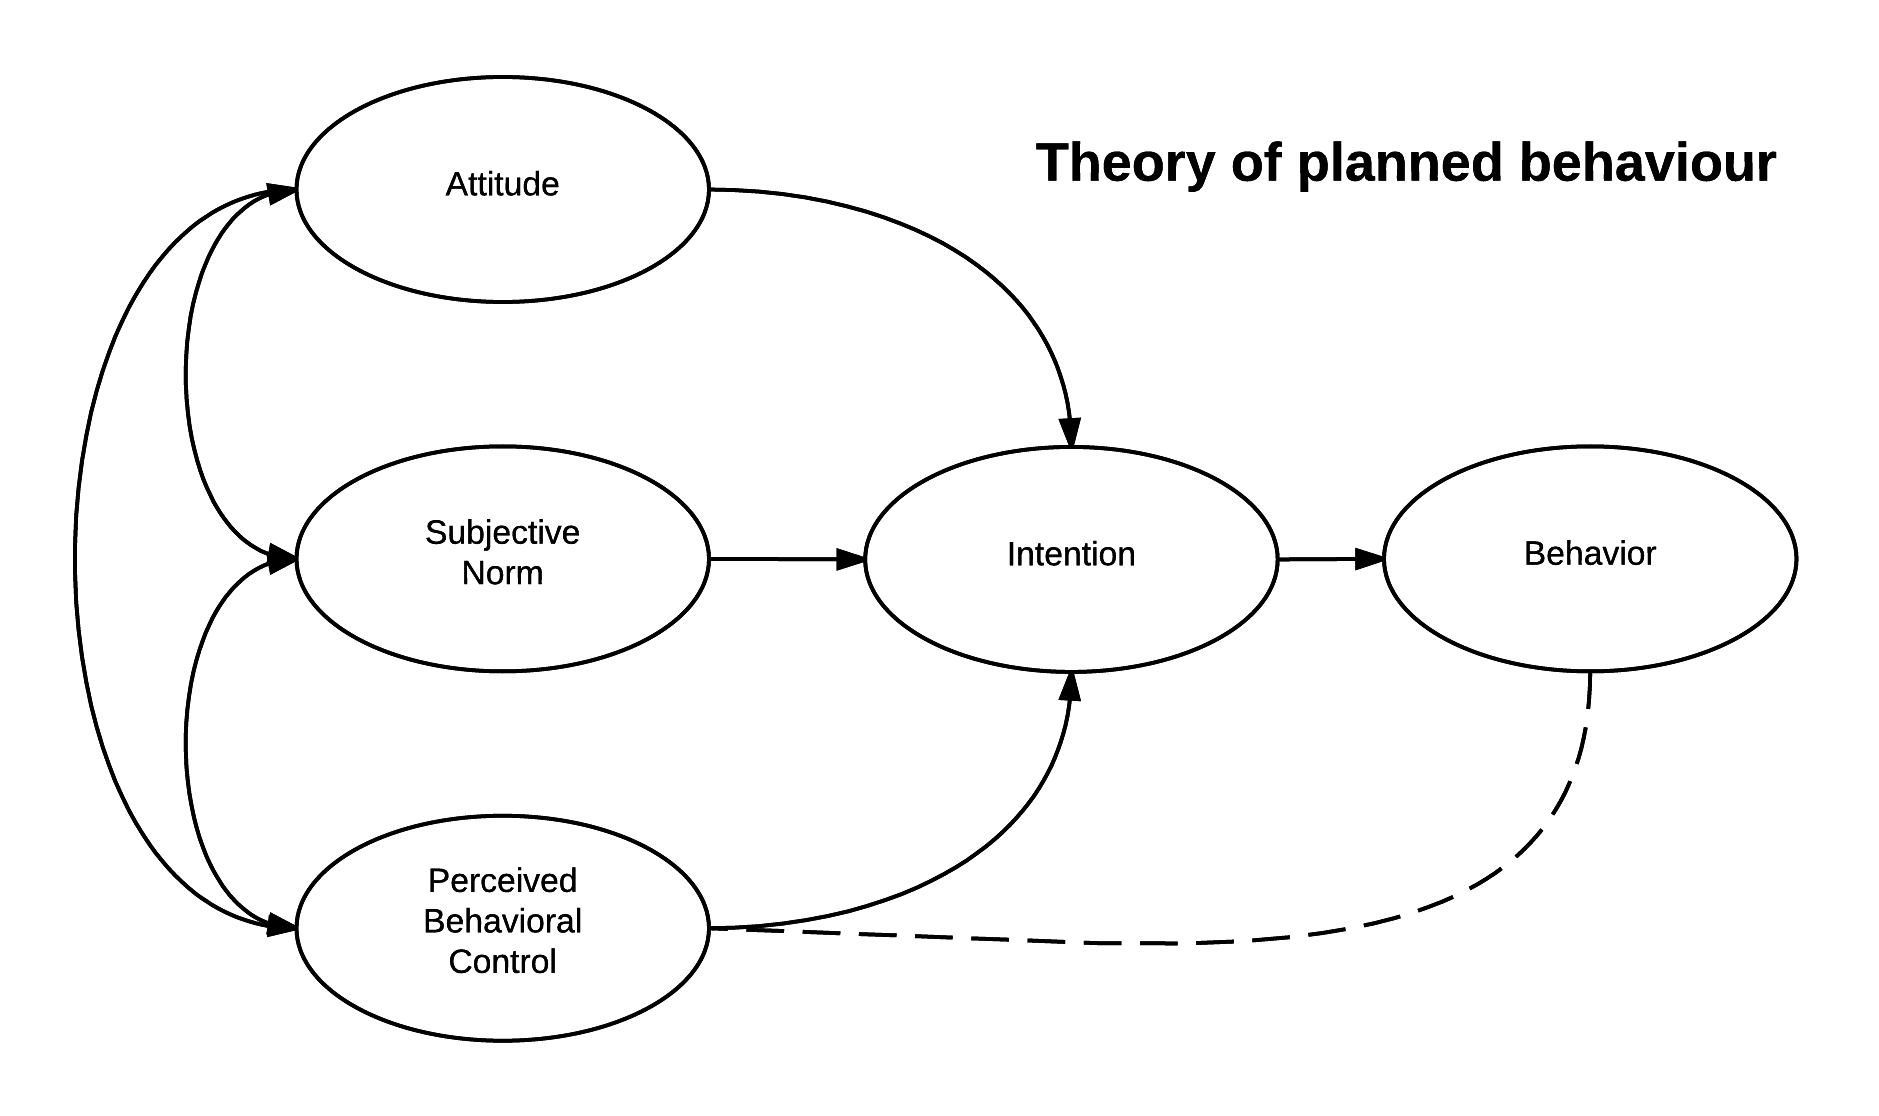
\includegraphics[width=0.8\textwidth]{Theory_of_planned_behavior_chart}}
%     \caption{ساختار نظریه رفتار برنامه ریزی شده
%       %\cite{kim2016integrated}
%     }
%     \label{fig:Theory_of_planned_behavior_chart}
%   \end{figure}\\

% \includepdf[pages={1}]{sexualityAgainstPopulation.pdf}

\begin{figure}[htpb]
    \centering
    \includegraphics[width=0.8\textwidth]{./img/sexualityAgainstPopulation.pdf}
    \caption{فراوانی جنسیت بیان شده در نمونه}
    \label{fig:sexualityAgainstPopulation}
\end{figure}

بعد از حذف داده‌های مربوط به آزمودنی‌هایی که اطلاعات مخدوش یا غیر قابل استفاده داشتند، تعداد
\CleanedSampleSize
باقی ماندند.

\section{سه‌گانه تاریک}
جدول 
\CompareDarkTriadStatisticsRef
به صور مقایسه‌ای 
شاخص‌های آماری میانگین و انحراف‌معیار به دست آمده در پرسشنامه پیاده شده در این آزمایش 
را با آزمایش‌های پیشین نمایش می‌دهد. 

\CompareDarkTriadStatisticsCustomTableCommand


\begin{landscape}
    \StyledTableFromDFCommand
\end{landscape}
% \includepdf[pages={1}]{./img/CorrPlotIntervals.pdf}
\begin{figure}[htpb]
    \centering
    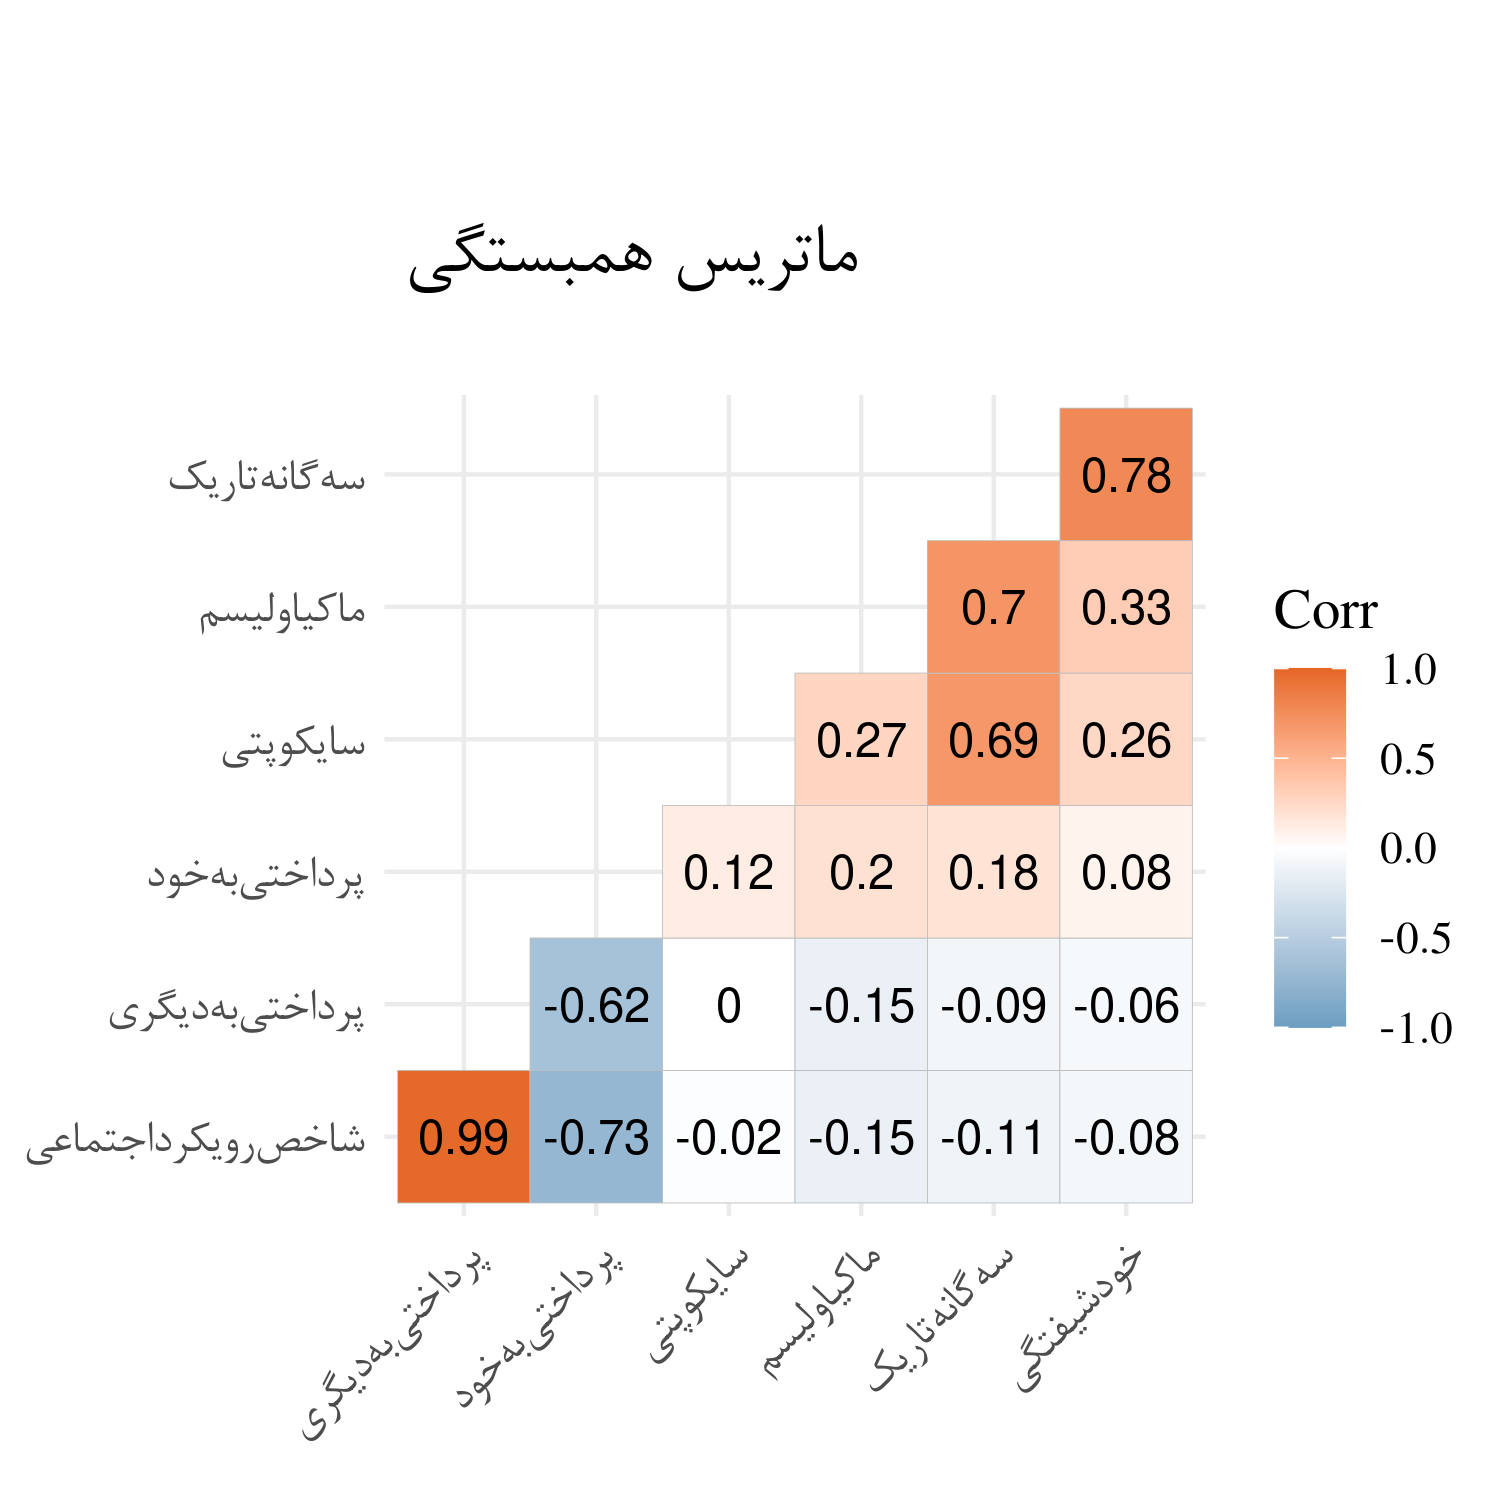
\includegraphics[width=0.8\textwidth]{./img/CorrPlotIntervals.png}
    \caption{ماتریس همبستگی}
    \label{fig:CorrPlotIntervals}
\end{figure}

% \subsection{نتایج آزمون جهت‌گیری ارزش اجتماعی}
\section{نتایج آزمون جهت‌گیری ارزش اجتماعی}
از میان همه شرکت کنندگان
\noOfIndividualisticParticipants
نفر در دسته
\textit{
    \gls{Individualistic}
}
،
\noOfCompetitiveParticipants
نفر در دسته
\textit{
    \gls{Competitive}
}
،
\noOfCooperativeParticipants
نفر در دسته
همکاری‌کننده
و
\noOfAltruisticParticipants
نفر در دسته
دیگر‌خواه
قرار داشتند.
(
تصویر \label{fig:SVOAgainstPopulation}
)

تصویر \label{fig:sexualityAndSVOAgainstPopulation}


\begin{figure}[htpb]
    \centering
    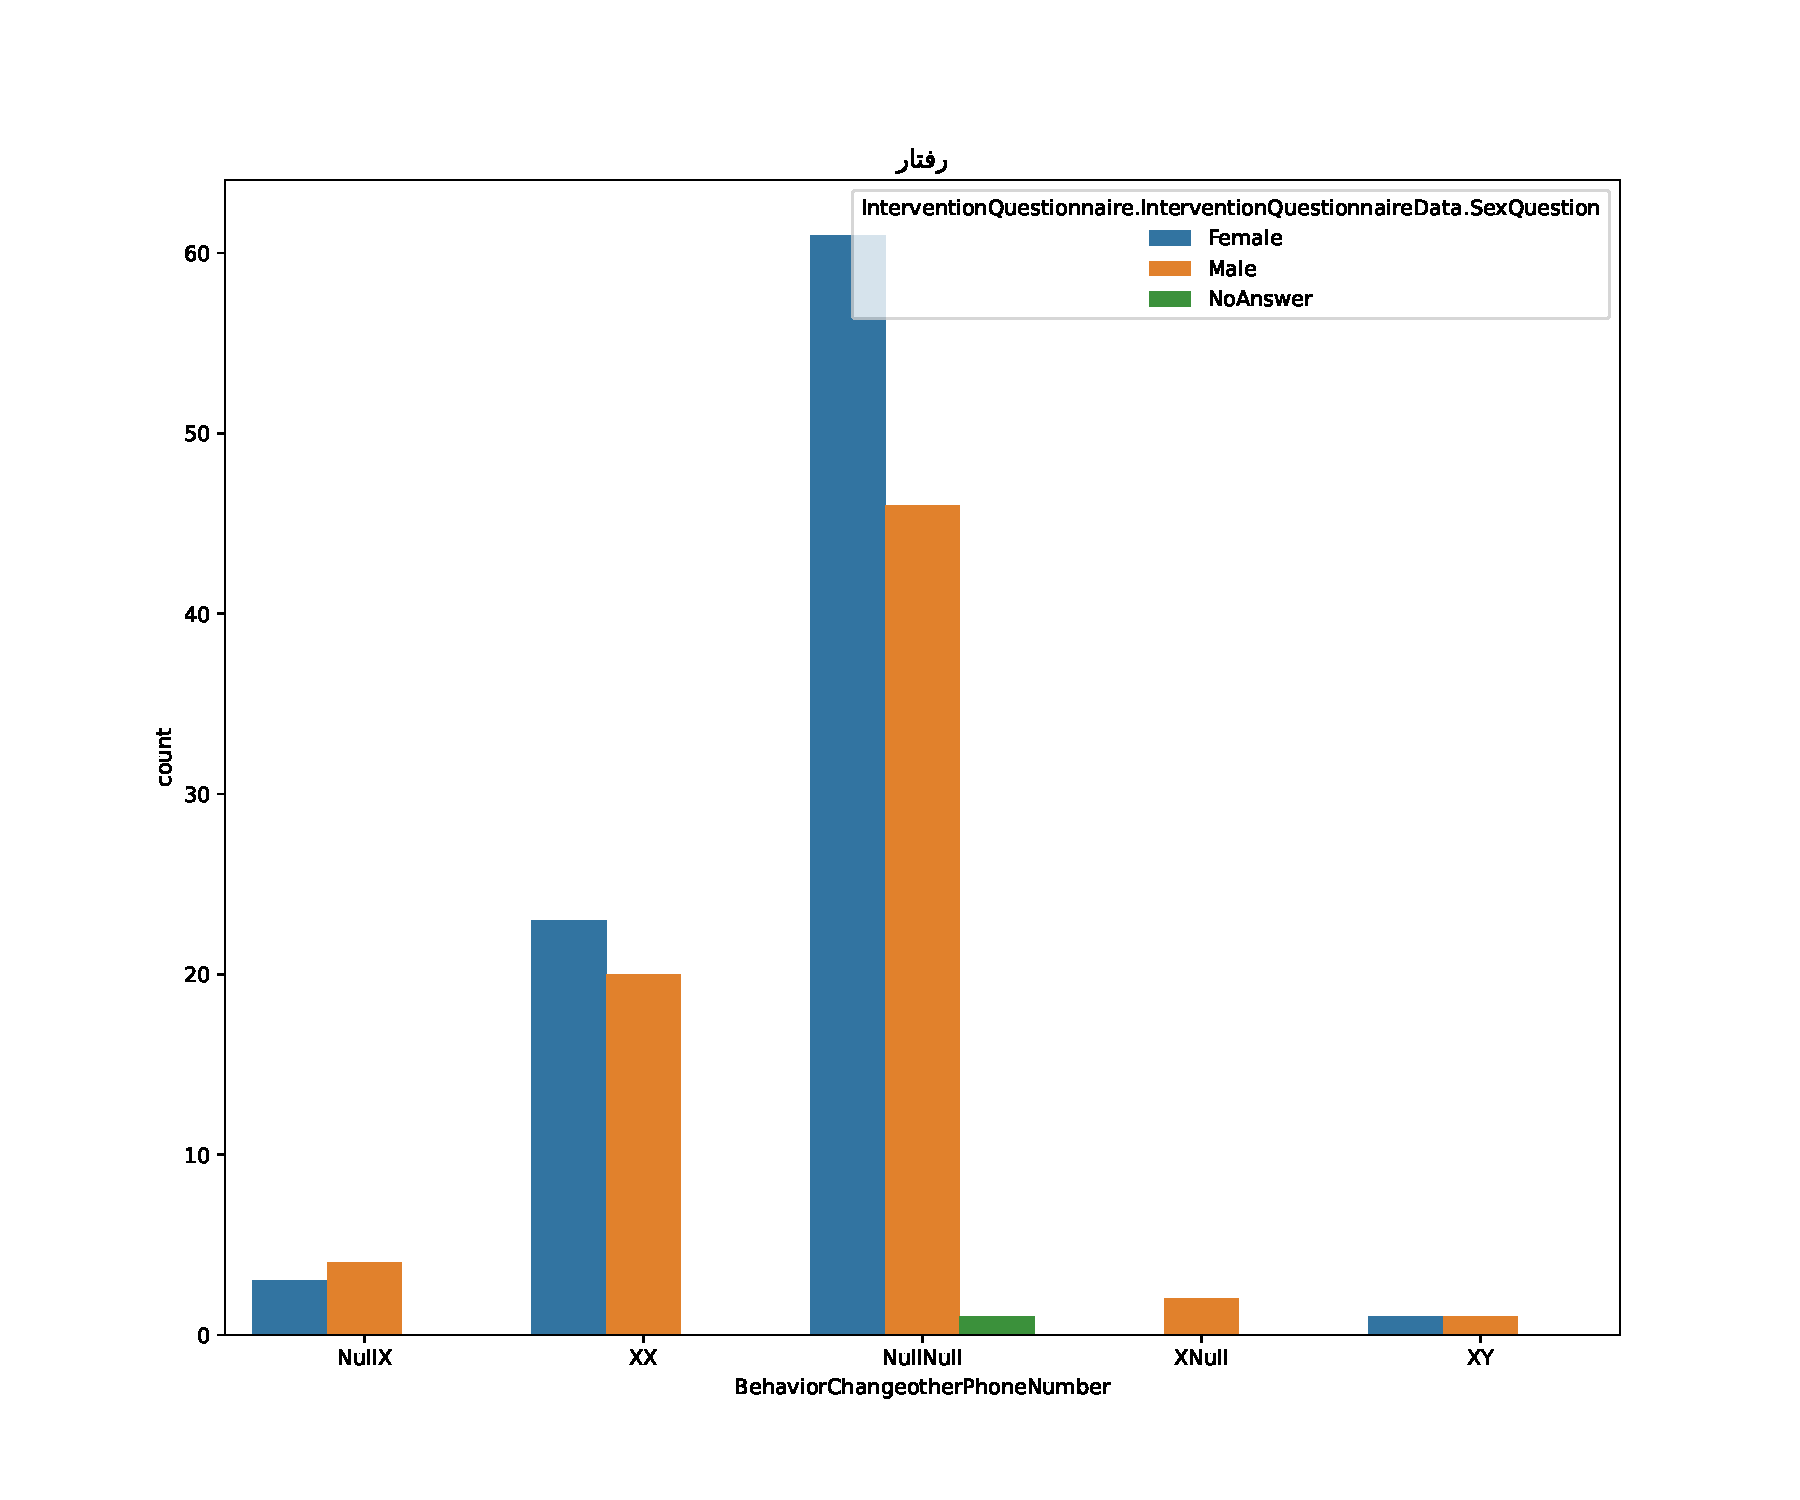
\includegraphics[width=0.8\textwidth]{./img/Frequency_Behavior_Phnone_Number.pdf}
    \caption{فراوانی جنسیت بیان شده در نمونه}
    \label{fig:Frequency_Behavior_Phnone_Number}
\end{figure}

فراوانی هر یک از رفتارها در
تصویر \label{fig:Frequency_Behavior_Phnone_Number}
مشخص است.

\begin{figure}[htpb]
    \centering
    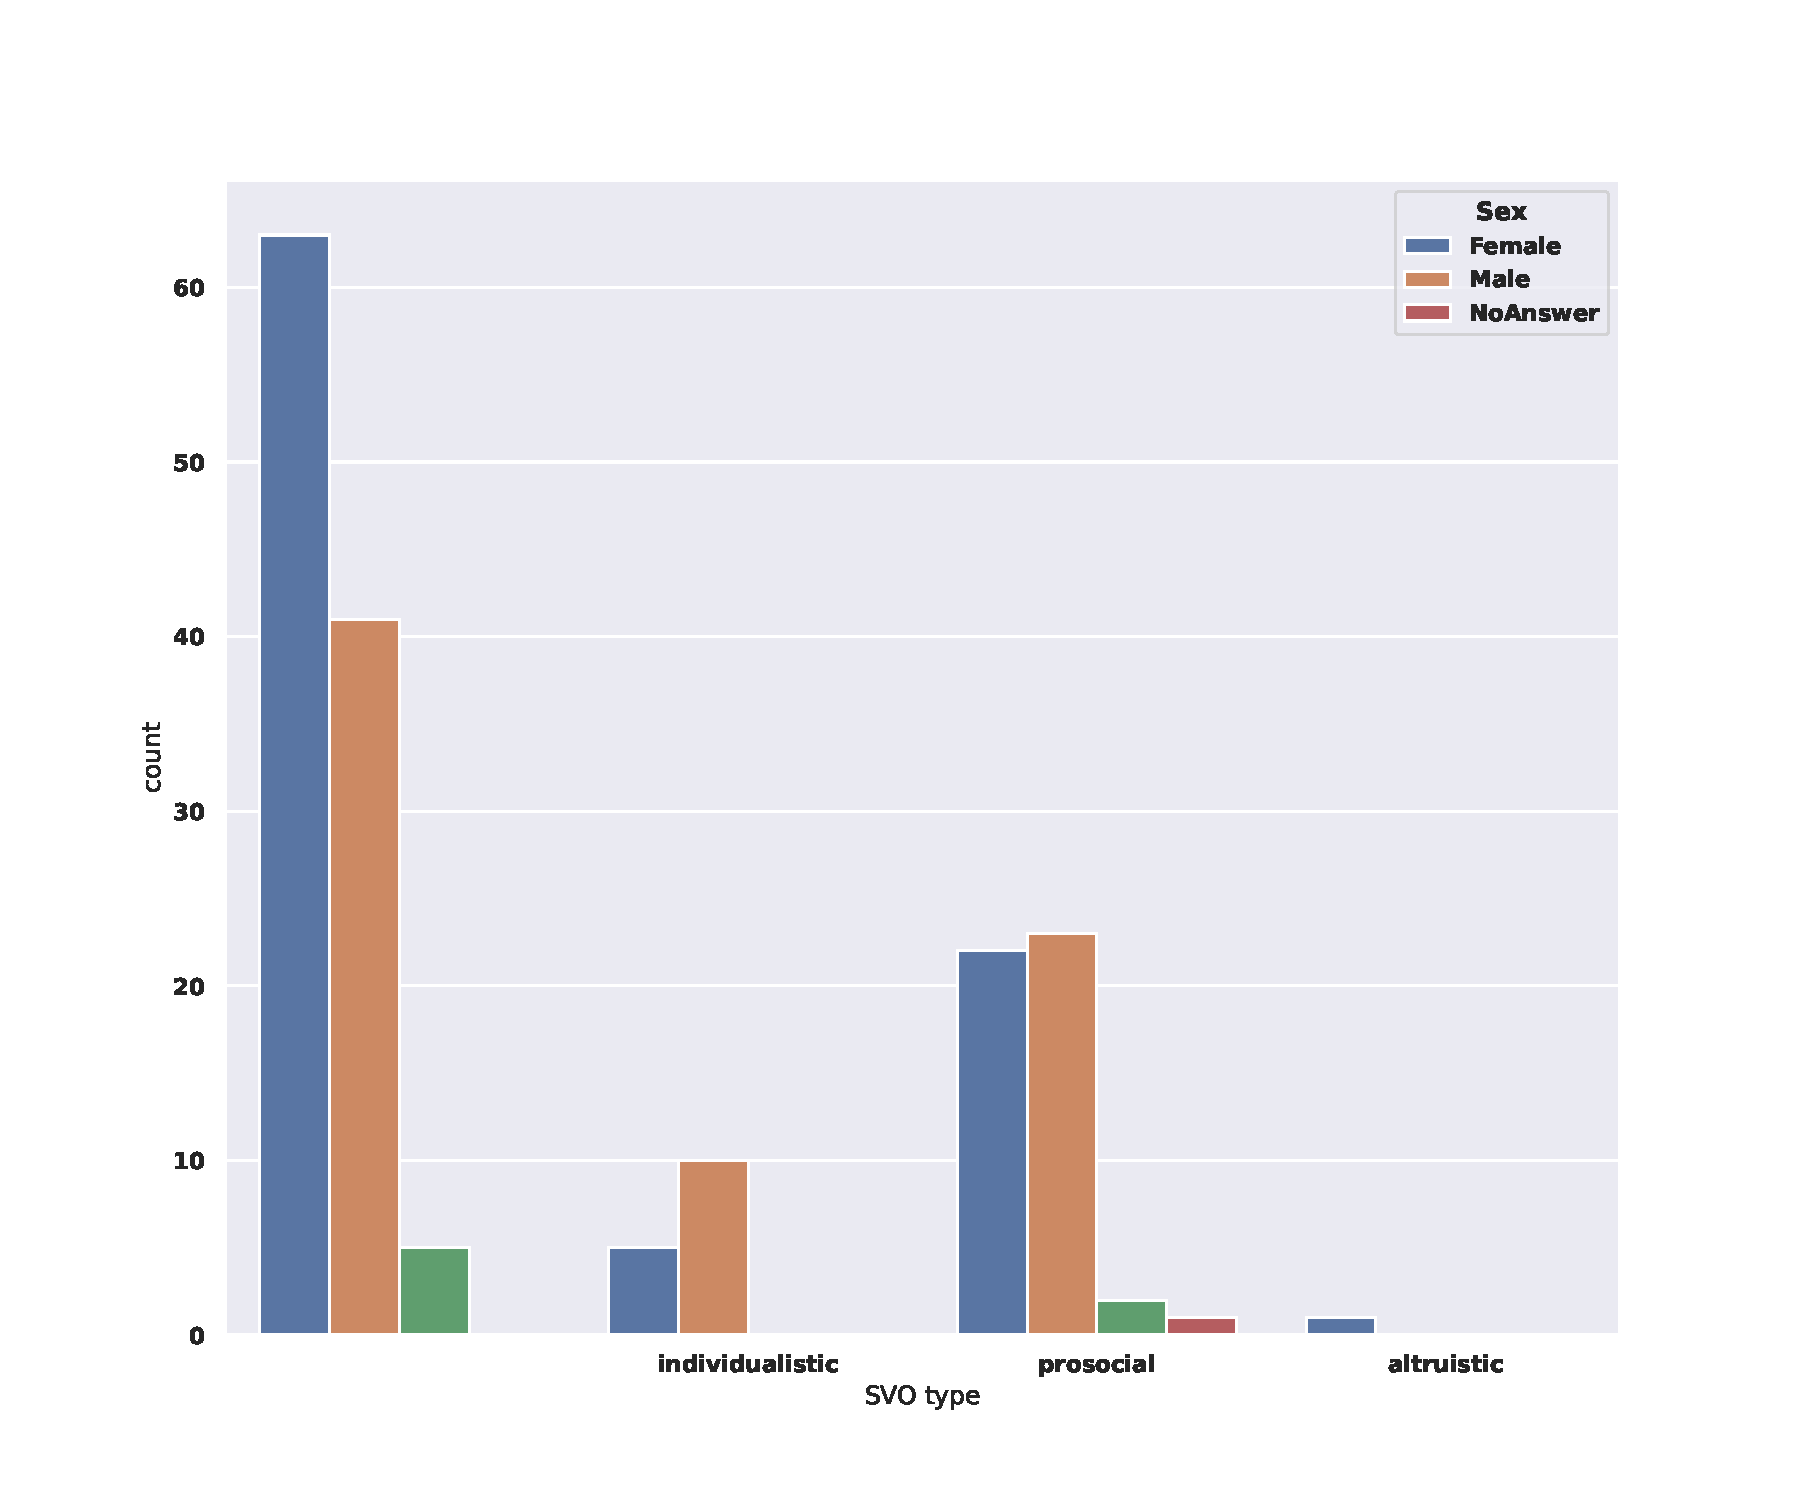
\includegraphics[width=0.8\textwidth]{./img/sexualityAndSVOAgainstPopulation.pdf}
    \caption{فراوانی دسته‌های رویکرد ارزش اجتمعای با توجه به جنسیت}
    \label{fig:sexualityAndSVOAgainstPopulation}
\end{figure}


\begin{figure}[htpb]
    \centering
    
\includegraphics[width=0.8\textwidth]{./img/SVOAgainstPopulation.pdf}
    \caption{فراوانی دسته‌های رویکرد ارزش اجتماعی}
    \label{fig:SVOAgainstPopulation}
\end{figure}
میانگین کلی نمره‌ای که همه آزمودنی‌ها در هر دو گروه به ۱۴ سوال هر دو دسته
نمرات از دید خود
\!(باور به ارزش اطلاعات)
\meanOfSelfWTPAllTwoParticipantGroupsAllTwoQuestionSection
با انحراف استاندارد
\SDOfSelfWTPAllTwoParticipantGroupsAllTwoQuestionSection
و از دید دیگران
\meanOfOtherWTPAllTwoParticipantGroupsAllTwoQuestionSection
\!(باور هنجاری به ارزش اطلاعات)
با انحراف استاندارد
\SDOfOtherWTPAllTwoParticipantGroupsAllTwoQuestionSection
بود.

\begin{figure}[htpb]
    \centering
    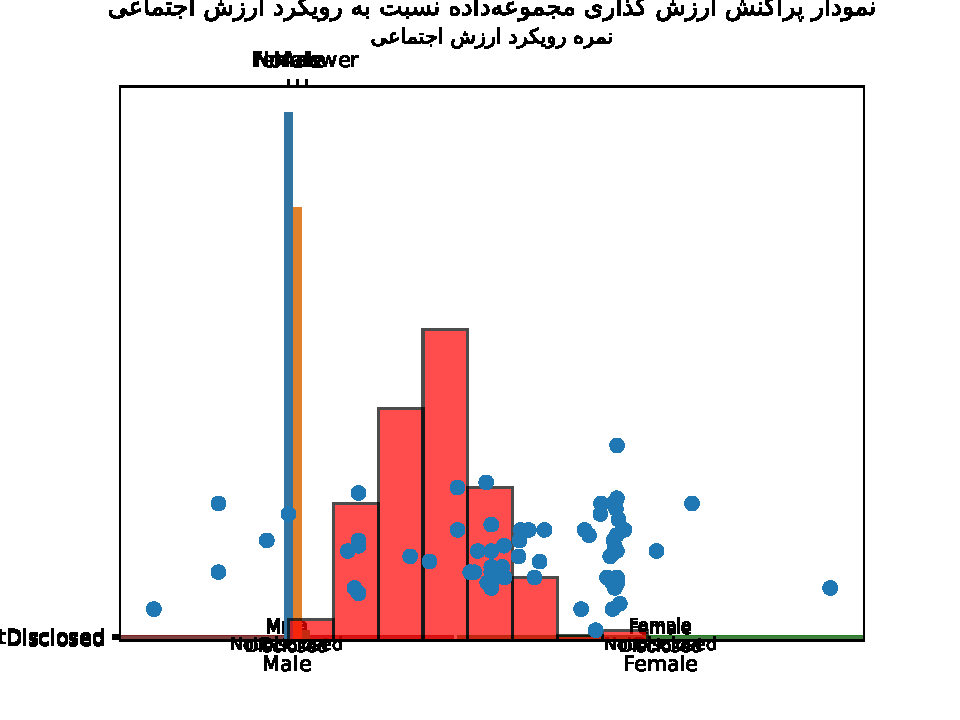
\includegraphics[width=0.8\textwidth]{./img/ScatterSVOScoreDarkTriadScore.pdf}
    \caption{نمودار پراکنش نمره رویکرد ارزش اجتماعی را نسبت به نمره سه‌گانه تاریک نشان می دهد. }
    \label{fig:ScatterSVOScoreDarkTriadScore}
\end{figure}
شکل
\label{fig:sexualityAndSVOAgainstPopulation}
نمودار پراکنش نمره رویکرد ارزش اجتماعی را نسبت به نمره سه‌گانه تاریک نشان می دهد.
و در شکل
\label{fig:SexToDTR}
فراوانی نمره‌های پرسشنامه سه‌گانه تاریک مشخس شده است.



\begin{figure}[htpb]
    \centering
    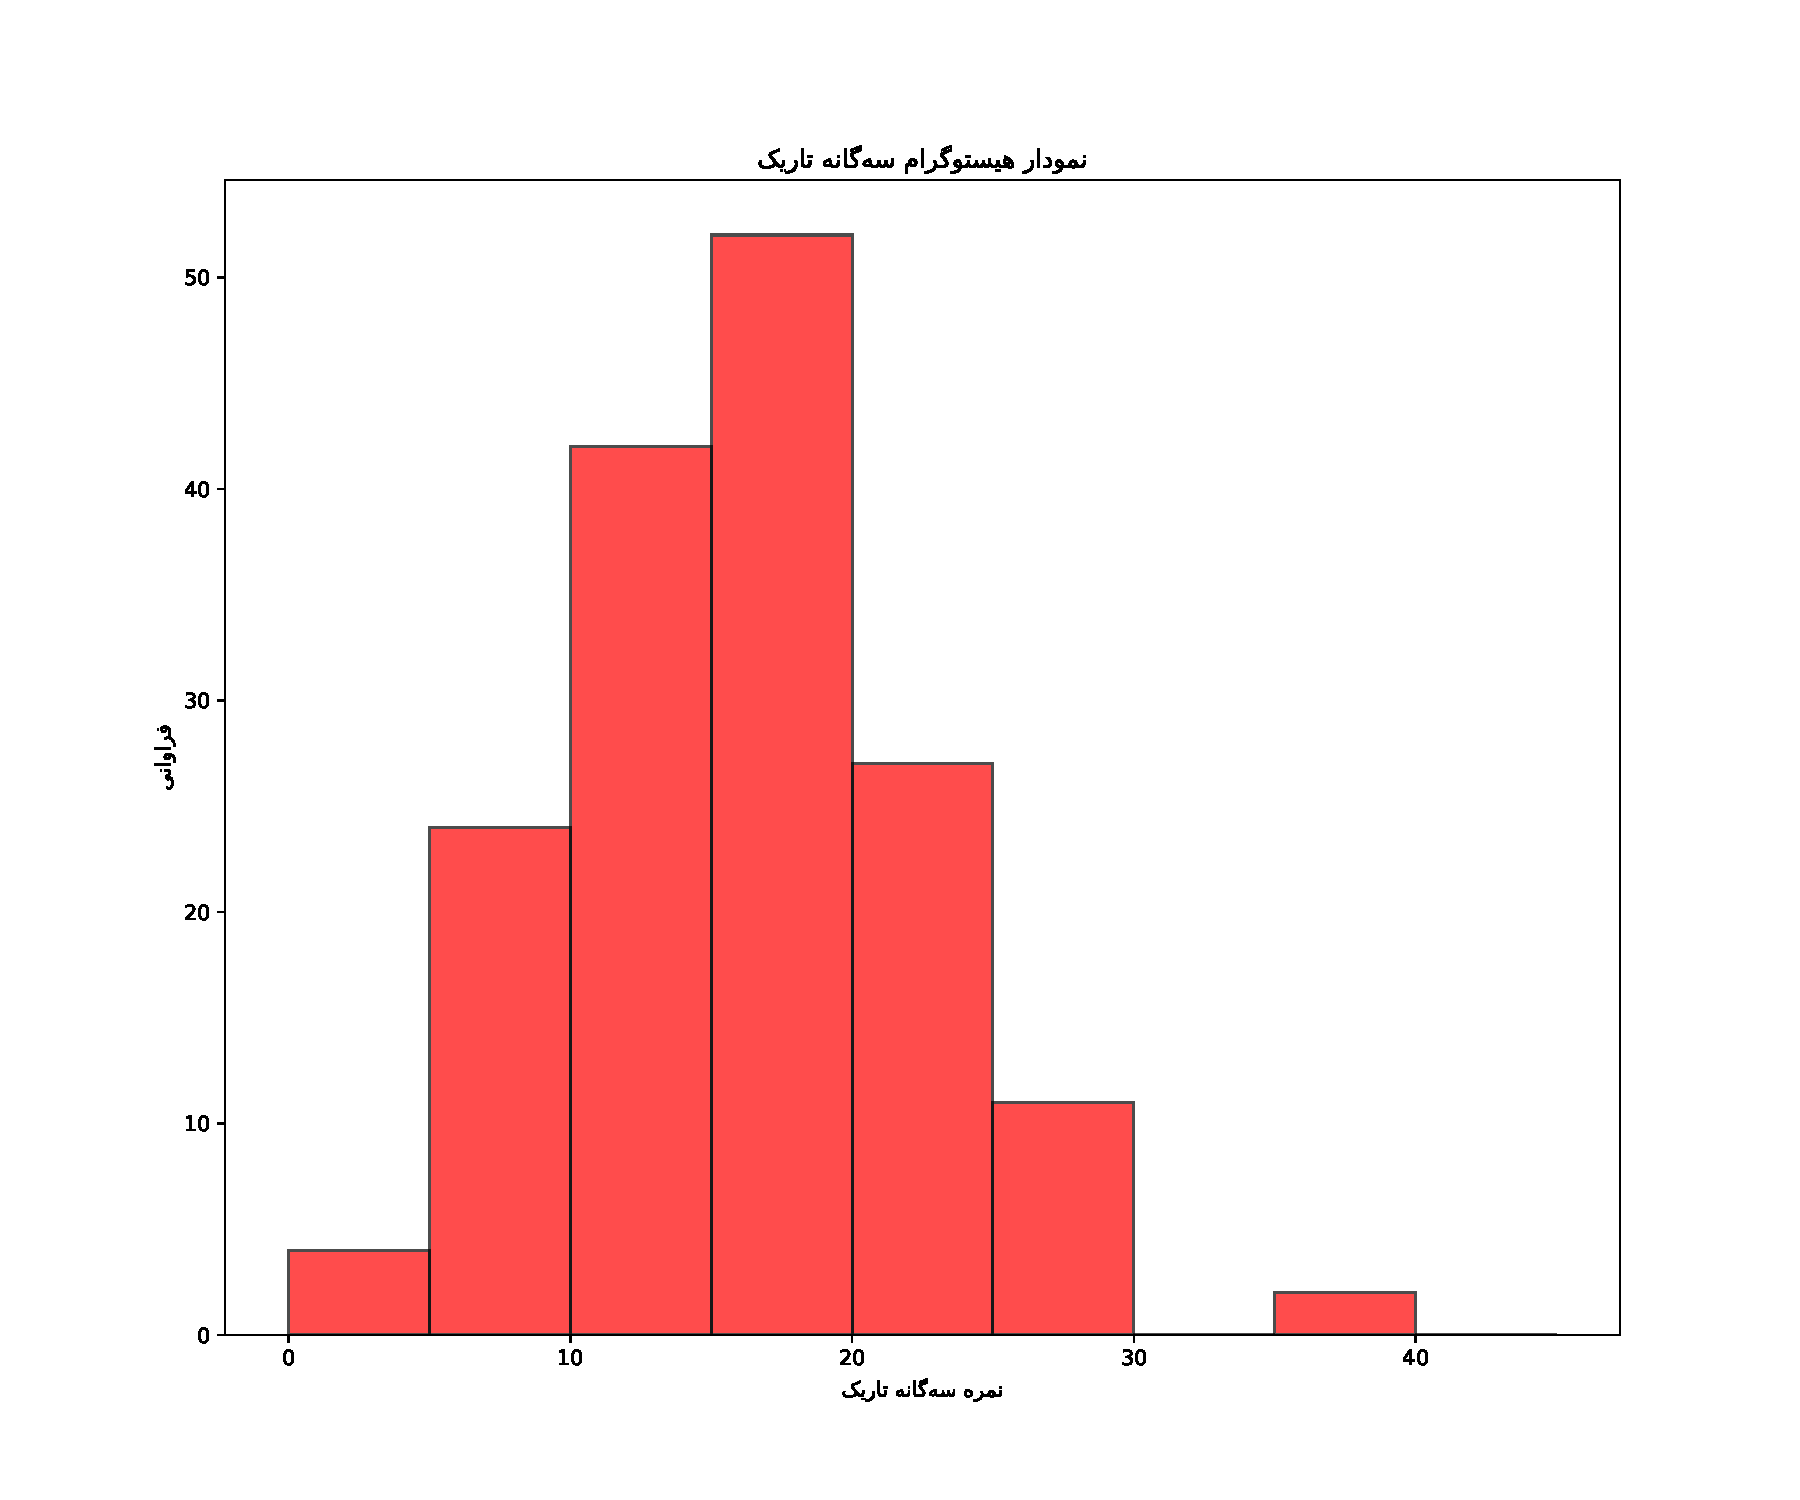
\includegraphics[width=0.8\textwidth]{./img/SexToDTR.pdf}
    \caption{نمودار پراکنش نمره رویکرد ارزش اجتماعی را نسبت به نمره سه‌گانه تاریک نشان می دهد. }
    \label{fig:SexToDTR}
\end{figure}


% \begin{table}[h!]
%     \begin{center}
%         \caption{More columns.}
%         \label{tab:table1}
%         \begin{tabular}{l|c|r|l}
%             \textbf{Value 1} & \textbf{Value 2} & \textbf{Value 3} & \textbf{Value 4} \\ % <-- added & and content for each column
%             $\alpha$         & $\beta$          & $\gamma$         & $\delta$         \\ % <--
%             \hline
%             1                & 1110.1           & a                & e                \\ % <--
%             2                & 10.1             & b                & f                \\ % <--
%             3                & 23.113231        & c                & g                \\ % <--
%         \end{tabular}
%     \end{center}
% \end{table}
% \subsection{پایایی پرسشنامه سیاهه ارزش‌گذاری مجموعه‌داده}
% میان نمرات به نیمه اول این پرسشنامه برای اندازه گیری
% باور به ارزش اطلاعات
% \!(ارزش‌گذاری از دید خود)
% \meanOfSelfWTPAllTwoParticipantGroupFirstQuestionSection
% با انحراف معیار
% \SDOfSelfWTPAllTwoParticipantGroupsFirstQuestionSection
% و نیمه دوم
% \meanOfOtherWTPAllTwoParticipantGroupsSecondQuestionSection
% \SDOfOtherWTPAllTwoParticipantGroupsSecondQuestionSection
% بود. با توجه به وجود
% %  عدم وجود
% همبستگی میان این دو نیمه
% (
% $
%     r=
%     \PiersonrValueForCorrelationBetweenFirstAndSecondPartOfQuestionsForSelfValuation
%     ,
%     P=
%     \PvalueForCorrelationBetweenFirstAndSecondPartOfQuestionsForSelfValuation
% $
% )
% این آزمون برای اندازه گیری باور به ارزش اطلاعات از دید خود در گروه‌های هفت‌گانه دارای پایایی درونی با
% روش نیمه‌سازی پرسشنامه است.
% همچنین با توجه به وجود
% %  عدم وجود
% همبستگی میان این دو نیمه
% (
% $
%     \!r=
%     \!\PiersonRValueForCorrelationBetweenFirstAndSecondPartOfQuestionsforOtherValuation
%     \!,
%     P=
%     \!\PvalueForCorrelationBetweenFirstAndSecondPartOfQuestionsForOtherValuation
% $
% )
% این آزمون برای اندازه گیری باور به ارزش اطلاعات از دید دیگری در گروه‌های هفت‌گانه دارای پایایی درونی با
% روش
% \textit{
%     \gls{Split Half}
% }
% پرسشنامه است.


% میانگین نمرات آزمودنی ها به دسته اول سوالات
\section{اعتبارسنجی}
% از طریق مقایسهٔ نتایج با نتایج کارهای دیگران، استفاده از روش‌های تحلیل پایائی
% \lr{(reliability)}
% و اعتبار
% \lr{(validity)}،
% نظرگیری از خبرگان
% \lr{(expert judgment or feedback)}
% و یا
% \lr{triangulation}
% انجام می‌شود.
